\section{\arch for OS Replacement}
Using containers to host applications becomes a common usage scenario 
in today's cloud~\cite{aws, gcpkubernetes, azureks, ibmkubernetes, vmwarepks}. 
Under this scenario, the act of OS replacement can be viewed as 
moving the state of all containers from the old VM with the 
stale OS to a new VM with the replacement OS. Again, we leverage 
intra-host live migration to avoid inter-host communication.

\subsection{Memory Translation for Containers}
The memory management for containers belongs to the above-mentioned single-level virtualization. As shown in \fref{fig:mappingc}, the page table of a process (belonging to a container) running in the VM stores the mappings between the guest virtual addresses (GVA) of the process and the guest physical addresses (GPA) of the VM. The hypervisor uses the EPT to map GPA to physical addresses (PA). 

\subsection{OS Replacement Overview}
To replace the stale OS for a container, the hypervisor creates a new VM with the replacement OS, and transfers the ownership of all the container's pages to this new VM.

\arch transfers the memory ownership using the \arch table, whose purpose is similar to that described for hypervisor replacement.
The  per-process \arch table stores the memory mappings from the pages of the container to the  pages of the physical memory, constructed by the stale OS, and is leveraged by the new OS for reconstructing the 
memory address space of the container during OS replacement. 

The replacement process on the new VM first reconstructs all the GVAs of the container. The VM kernel then allocates corresponding GPAs and sets up the GVA-to-GPA page mappings in the page table of the container. Finally, the new VM's kernel invokes a series of \texttt{hypercall\_map} hypercalls to the hypervisor, which installs the GPA-to-PA page mappings in the new VM's EPT table using the \arch table.

The transfer of execution control is performed as follows:
The container's execution is paused at the stale OS
and its execution state (all state of the container) 
are transferred to the replacement VM's control, which then resumes execution of the new VM. Finally, once the control of the container is transferred to the replacement OS, 
the stale OS can unmap the container's memory from its address space and be safely deprovisioned. 

\begin{figure}[t!]
 	  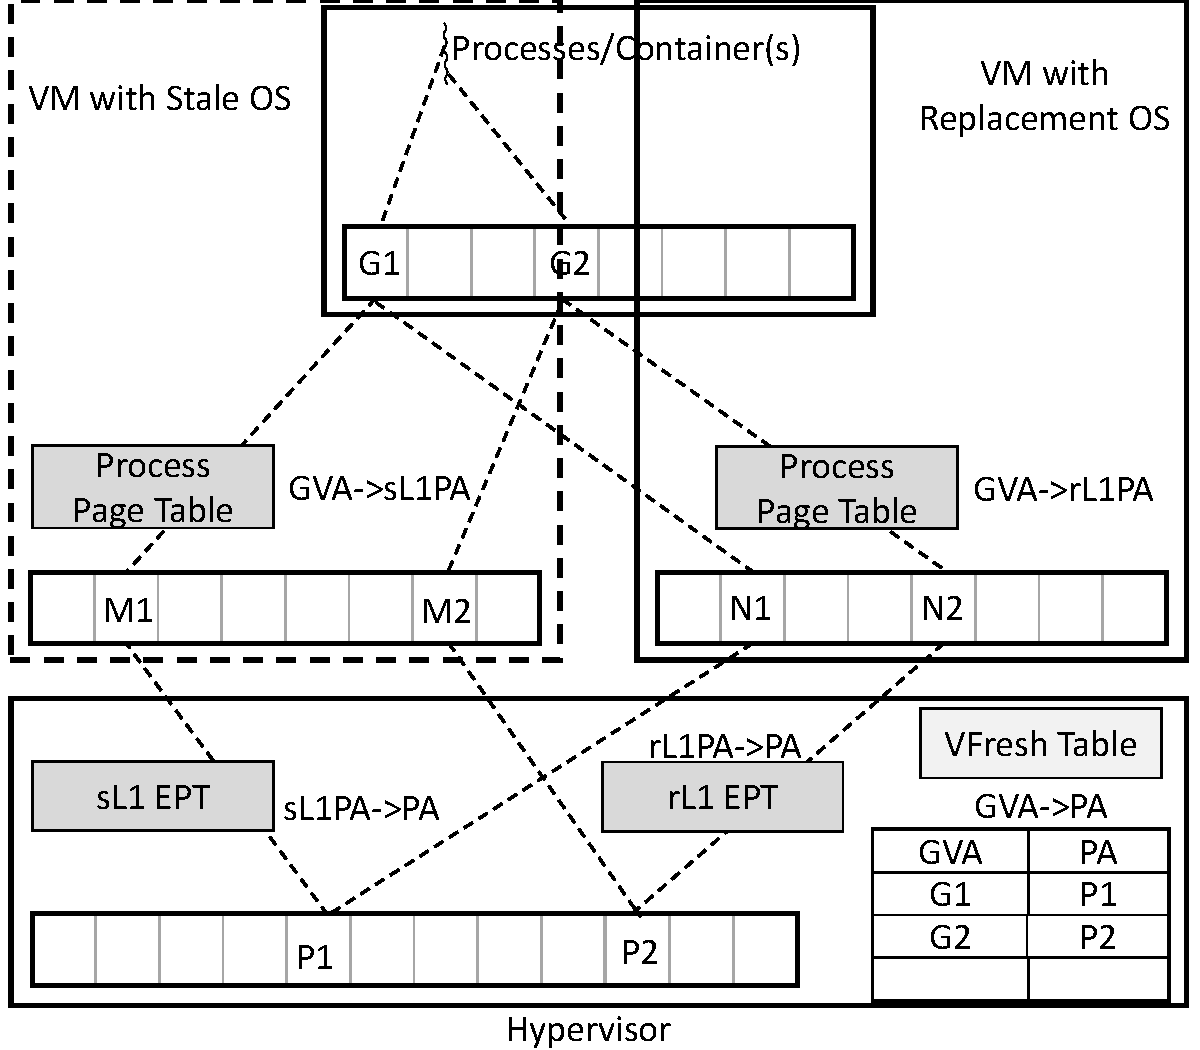
\includegraphics[width=0.45\textwidth]{figures/vfresh-table-container.pdf}
  \caption{Memory translations for OS replacement.}
  \label{fig:mappingc}
  %\includegraphics[width=15cm,height=6cm,keepaspectratio]{architecture__1_.jpg}
  \vspace{0.2in}
\end{figure}


%Essentially, a container consists of a hierarchy of processes as well as isolation mechanisms (e.g., \texttt{cgroups} and \texttt{namespaces} in Linux). If not specified, processes running upon an OS belong to a default container. Hence, moving a container from one VM to another for OS replacement needs to copy the state of all processes in the container from one VM to another. Again, \arch's OS replacement relocates the memory ownership of all processes instead of copying memory data. The design of \arch's OS replacement is  similar to the above hypervisor replacement, and we focus on the differences in the OS replacement.




    
%\subsection{OS Switching}
%During OS replacement, the stale VM's kernel provides the GVA-to-GPA page mappings for \texttt{hypercall\_put} hypercalls to build an \arch table. Such mappings can be obtained by walking through the page table of the process in the stale VM's kernel. These mappings can also be obtained using a user-level replacement tool (e.g., CRIU~\cite{criu}), which dump and transfer memory state from the user space (e.g., reading from \texttt{$\slash$proc$\slash$[PID]$\slash$pagemap}). To support such a user-level live OS replacement implementation, \arch provides a new system call, \texttt{syscall\_set}, which takes a list of GVA-to-GPA mappings from the user space. Thus, in this syscall, the VM kernel simply passes received GVA-to-GPA mappings to the hypervisor via \texttt{hypercall\_put} hypercalls.  

%The replacement process on the new VM with the replacement OS first reconstructs all the GVAs (e.g., with the \texttt{mmap} system call). The VM kernel then allocates corresponding GPAs and sets up the GVA-to-GPA page mappings in the page table of the process (e.g., with the \texttt{set\_pte\_at} system call). Finally, the new VM's kernel invokes a series of \texttt{hypercall\_map} hypercalls to the hypervisor, which installs the GPA-to-PA page mappings in the new VM's EPT table using the \arch table as stated above. 

%To further support user-level live OS replacement implementations, which dump and transfer memory state from the user space (e.g., CRIU \cite{criu}), \arch provides a  system call, \texttt{syscall\_set}. Similar to \texttt{hypercall\_set}, \texttt{syscall\_set} takes a list of GVA-to-GPA mappings from the user space. Differently, the user-level replacement tool should prepare these mappings (e.g., reading from \texttt{$\slash$proc$\slash$[PID]$\slash$pagemap}). Thus, in this syscall, the VM kernel simply passes received GVA-to-GPA mappings to the hypervisor via \texttt{hypercall\_set} hypercalls.  

%Using a memory copying based approach, reconstructing address space of the process on the VM with the replacement OS involves two steps: (1) creating the same GVAs (e.g., via \texttt{mmap}) as that of the process on the stale VM (from received memory mapping metadata); and (2) loading memory page contents (e.g., via \texttt{preadv}) from the received memory data. With given GVAs, loading memory page contents will establish all the mappings in two page tables --- the GVA-to-GPA page table of the process and the GPA-to-PA EPT of the VM with the replacement OS.


%\label{sec:destdesign}
%This syscall also needs to change the virtual address of the array passed from the user space to a set of disjoint GPAs before calling hypercalls). 
%\end{itemize}

%\begin{figure}[t!]
%  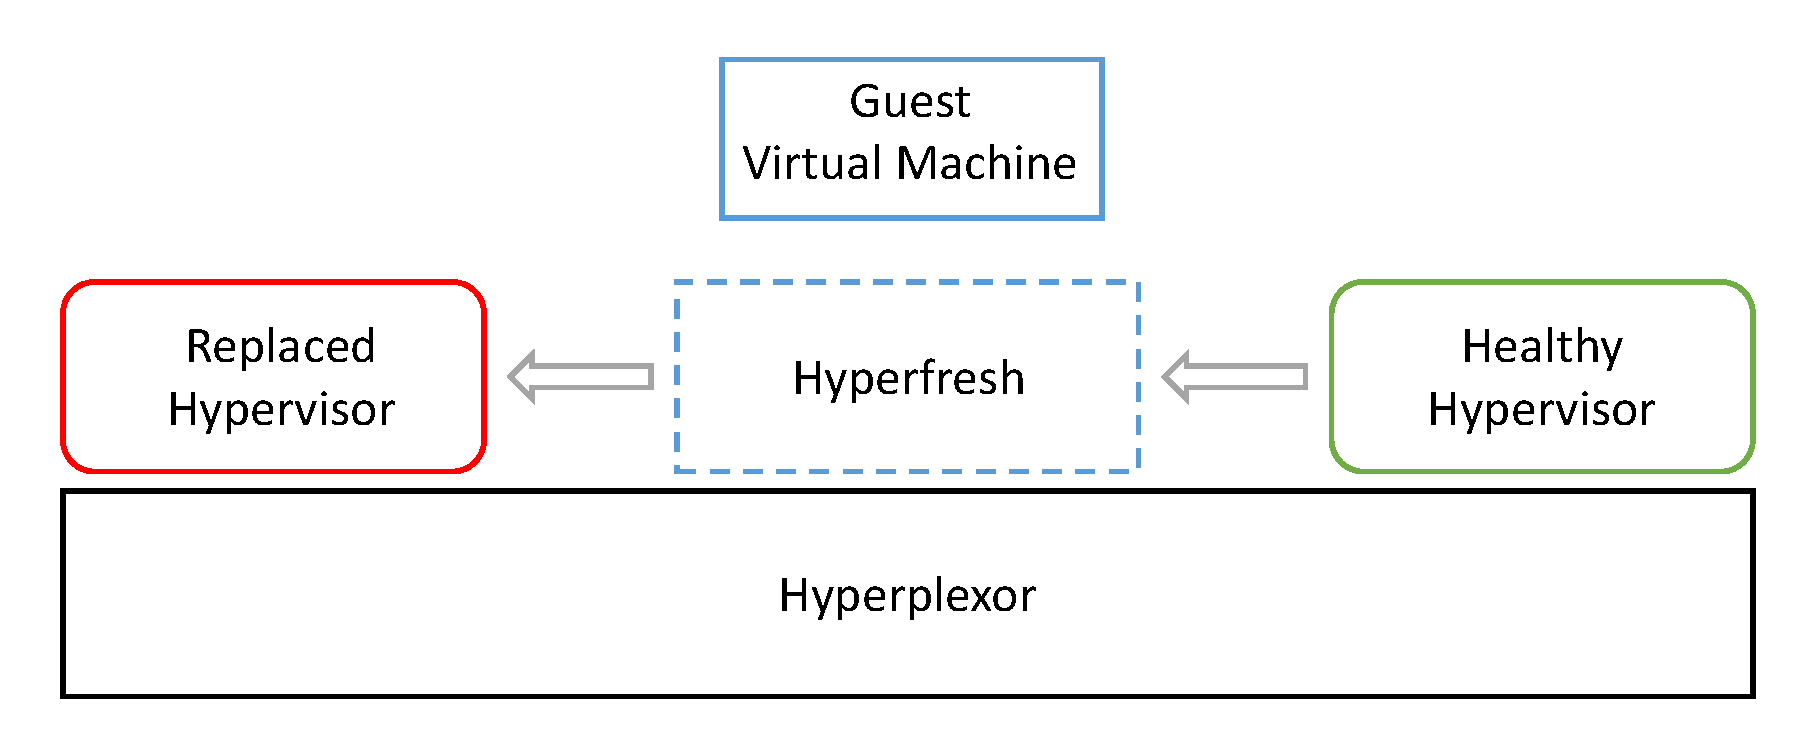
\includegraphics[width=0.5\textwidth]{figures/shift.pdf}
%  \caption{Hypervisor switching operation}
%  \label{fig:switching}
  %\includegraphics[width=15cm,height=6cm,keepaspectratio]{architecture__1_.jpg}
%\end{figure}

%\subsection{Hypervisor Switching}
%The guest initially runs on the hypervisor which in turn runs on thin hyperplexor. The guest pre-allocates it's memory by pinning the pages in memory during boot time. When the current hypervisor requires updates, a new hypervisor with pre-installed updates boots up  and runs the guest in migration state. The guest in migration state maps it's memory in advance to the guest running on current hypervisor using grant table mechanism described above and waits for the VCPU and I/O device state. The guest on current hypervisor is then paused and the VCPU and I/O device state are transferred to the guest on updated hypervisor as shown.

\subsection{Implementation Details}
We have implemented an OS replacement prototype based on CRIU \cite{criu} --- a well-known checkpoint/restore tool implemented in the user space. CRIU consists of two stages: checkpointing (on the source VM) and restoration (on the destination VM). By automating these two parts, we implemented the live OS replacement for containers. \arch's OS replacement operation involves the transfer of all the state of containers and their processes (e.g., file descriptors, memory maps, registers, namespaces, cgroups, etc.) except for memory content from the source VM (with the stale OS) to the destination VM (with the replacement OS).

In our implementation, when the OS replacement operation is invoked, one of the target processes in a container is paused. During the checkpointing phase, \arch collects all state of the process except for its memory content and build the \arch table. During the restoration phase, \arch restores the process state on the destination VM and relocates the memory ownership. In the final stage, \arch resumes running the process on the destination VM. The source VM unmaps the pages of the process from its address space. \arch repeats this process until all target processes are moved to the destination VM. Then the source VM can be gracefully shutdown. 

\para{The \arch Table.}
To build the \arch table for OS replacement, the hypervisor needs a list of GVA-to-GPA page mappings of a container from the stale OS. Similarly to the hypervisor replacement, \arch invokes multiple \texttt{hypercall\_put} hypercalls to pass a list of GVA-to-GPA page mappings to the hypervisor. For each received GVA-to-GPA page mapping, the hypervisor translates the page of GPA to the page of PA (i.e., using the VM's EPT), and puts the corresponding GVA-to-PA page mapping to the {\em \arch table}.

Restoring the address space of a container on the new VM needs to build GVAs, GPAs, and their mappings. Given the GVA-to-GPA page mappings of the container, the new VM's kernel invokes multiple \texttt{hypercall\_map} hypercalls to pass a list of GVA-to-GPA page mappings of the container to the hypervisor. 
For each received GVA-to-GPA page mapping, the hypervisor: (1) looks up the {\em \arch table} to find the GVA-to-PA page mapping with GVA as the key; and (2) installs the GPA-to-PA page mapping in the EPT page table of the new VM. 
%Similarly, the new VM's kernel can invoke multiple \texttt{hypercall\_map} hypercalls to pass all GVA-to-GPA mappings for fully relocating memory address space for the process on the new VM with the replacement OS.  

\para{Checkpointing.}
We modified CRIU's checkpointing code to replace the procedure of dumping memory content with the one which builds the \arch table by calling \arch's new system call, \texttt{syscall\_set}. The function takes an array of GVAs and the their mapped GPAs (e.g., reading from the \texttt{/proc/[PID]/pagemap} file).
%which stores the GVA-to-GPA mappings. 
We further use the \texttt{memalign} function to allocate page-size aligned memory for the input arrays. The \texttt{syscall\_set} system call translates the base address of the two arrays (containing GVAs and GPAs) into GPAs, and invokes the \texttt{hypercall\_set} hypercall to transfer the GPAs of the arrays to the hyperplexor.  
As stated above, the \texttt{hypercall\_set} hypercall obtains the GVA-to-PA mappings, and inserts them to the \arch table.

\para{Restoration.} On the destination VM, we modify CRIU's restoration code to replace the procedure of loading memory content with the one of transferring address space via \arch's new system call, \texttt{syscall\_map}. Before invoking  \texttt{syscall\_map}, the restorer needs to restore GVAs using the \texttt{mmap} system call. It then invokes \arch's \texttt{syscall\_map} to pass an array of GVAs. The \texttt{syscall\_map} system call in turn gets free VM memory pages, GPAs, and establish the GVA-to-GPA page mappings in the process's page table. With such GVA-to-GPA page mappings, the \texttt{syscall\_map} system call invokes the \texttt{hypercall\_map} hypercall to transfer these mappings to the hypervisor. As stated above, the \texttt{hypercall\_map} hypercall installs the GPA-to-PA page mappings in the destination VM's EPT table.

